\documentclass[output=paper]{langsci/langscibook} 
\ChapterDOI{10.5281/zenodo.2579049}

\title{Cross-lingual linking of multi-word entities and language-dependent learning of multi-word entity patterns} 

\author{Guillaume Jacquet\affiliation{European Commission, Joint Research Centre, Ispra, Italy}\and Maud Ehrmann\affiliation{Swiss Federal Institute of Technology in Lausanne (EPFL) -- Digital Humanities Laboratory}\and Jakub Piskorski\affiliation{European Commission, Joint Research Centre, Ispra, Italy}\and Hristo Tanev\affiliation{European Commission, Joint Research Centre, Ispra, Italy}\lastand Ralf Steinberger\affiliation{European Commission, Joint Research Centre, Ispra, Italy}}

\lehead{G. Jacquet, M. Ehrmann, J. Piskorski, H. Tanev \& R. Steinberger}
\shorttitlerunninghead{Cross-lingual linking of multi-word entities and learning of entity patterns}


% \epigram{Change epigram in chapters/01.tex or remove it there }

\abstract{The contribution of our work is to address multi-word entity (MWEntity) recognition in a highly multilingual environment. The first part of this chapter describes completed work on recognising MWEntities in large volumes of text in 22 different languages, on identifying monolingual variants for the same entity and on linking the equivalent groups of variants across all languages. The second part describes ongoing work on learning MWEntity recognition rules based on the already recognised MWEntities, using distributional patterns. This rule-learning approach, which has currently been tested only for English and Spanish, does not require linguistic tools such as part-of-speech taggers so that it is perfectly suitable for our highly multilingual environment. When adding these learnt patterns to an existing rule-based Named Entity Recognition (\textsc{ner}) system, F1 performance for Spanish increases from 42.4\% to 50\% (18\% increase) and for English from 43.4\% to 44.5\% (2.5\% increase). The purpose of our effort is to improve on current methods for Named Entity Recognition (\textsc{ner}) in order to turn free text into semi-structured data that can be used for improved search, for linking related news over time and across languages, for trend detection and – more generally – for a more advanced intelligent analysis of large volumes of multilingual text collections.}

\maketitle
\begin{document}

\section{Introduction} 
%\remMaud{as discussed on skype, I liked the initial generic frame formulated by Ralf on going from unstructured to structured data/information to answer the needs of applications xyz.}

%In this chapter, we present our contribution in addressing multi-word entity (MWEntity) recognition in a highly multilingual environment. The first part of this contribution describes completed work on recognising MWEntities in large volumes of text in 22 different languages, on identifying monolingual variants for the same entity and on linking the equivalent groups of variants across all languages. The second part describes our ongoing work on learning MWEntity recognition rules based on the already recognised MWEntities. We then show how such rules can improve the recognition of new or unknown MWEntities. The purpose of our effort is to improve on current methods for Named Entity Recognition (\textsc{ner}) in order to turn free text into semi-structured data that can be used for improved search, for linking related news over time and across languages, for trend detection and – more generally – for a more advanced intelligent analysis of large volumes of multilingual text collections.

%by addressing the specific case of multi-word entities.

Named Entities (NEs) such as persons, organisations, locations and events are major bearers of information in text as they provide answers to the text representation questions \textit{Who did What to Whom, Where and When}. For this reason, work on \textsc{ner} and Classification is abundant \citep{nadeau-05} and NEs have been linked to knowledge bases \citep{rao-13,mcnamee-09}. Major challenges are homographic entity names belonging to different classes or within the same class and the existence of variant spellings within the same or across different languages, as well as morphological inflection \citep{steinberger-13}. An additional challenge for names of organisations and events is that they may be referred to as multi-word expressions or acronyms, e.g., \textit{Economic Community of West African States} (abbreviated as ECOWAS), and that name parts are likely to be translated, e.g., the equivalent Portuguese \textit{Comunidade Económica dos Estados da África Ocidental} (abbreviated as CEDEAO). Users searching for such an entity will want to retrieve all mentions, independently of their spelling or abbreviation or language.

Our interest in entity variants originally stems from our multiannual work on the Europe Media Monitor (EMM), which is a freely accessible meta-news web platform\footnote{See \url{http://emm.newsbrief.eu/overview.html} and \url{http://emm.newsexplorer.eu/}} that has been online since 2002 \citep{steinberger-09,steinberger-15}. EMM currently gathers an average of 300,000 news articles per day in about 70 languages from about 8,000 news websites (HTML pages and RSS feeds). News items are classified into thousands of categories 
%(more than half are customer-specific so that they are not available on the public website)
 and related news (e.g., from different news sources) are grouped into clusters. EMM-NewsBrief and the \textit{Medical Information System} EMM-MedISys group the newest articles every ten minutes and show intra-day trends, while EMM-NewsExplorer groups related articles published on the same calendar day and follows trends over longer periods of time. For each news article and for each news cluster, the system displays extracted meta-information, which includes the news category, entity names found (persons, organisations and geo-locations), quotations by and about entities, as well as various types of statistics, trends and analysis results. Entity mentions are disambiguated according to entity types (e.g., \textit{Paris Hilton} is a person) and geographical reference (e.g., there are about fifteen places world-wide called \textit{Paris}). Spelling variants of the same person or organisation name are mostly recognised as belonging to the same real-world entity. For instance, the spellings \textit{Jean-Claude Juncker, Jean Cloud Junker, Jean-Claude Juencker, Жан-Клод Юнкер, Ζαν Κλοντ Γιούνκερ} % \remGuillaume{TODO: Must display properly chinese and arabic scripts} جونكر كلود جان, Ζαν Κλοντ Γιούνκερ, 让-克洛 德•容克}
and many others are all identified as referring to the 12th President of the European Commission. Such multilingual entity variants – and also disambiguated place names – are a major ingredient for the successful identification of related news across languages in EMM-NewsExplorer. The system was entirely developed by the European Commission’s Joint Research Centre (JRC) with the purpose of providing media monitoring functionality for the European institutions, for national authorities of the European Union (EU) Member States, for international organisations such as the United Nations or the African Union, as well as for EU partner country organisations. However, the results are also freely accessible to the wider public through web pages and as customisable mobile applications.

 
%TODO : maybe remove the two next paragraphs
%In recent years, EMM’s text mining capacity has also been applied to social media posts (e.g., \citealt{Zavarella-14}) and to documents resulting from generic web searches \citep{Crawley-10}, thus widening the range of analysed text types. \textsc{ner} software does not perform equally well on all text types. We try to overcome this limitation by building up a large historical collection of names previously seen in hundreds of millions of news articles (known names) that can then be recognised through a simple lookup rather than re-recognising the names anew in every text. This should allow a decent performance even for poorly written texts such as Twitter messages. Accumulated lists of variants within the same and across different languages and scripts additionally have the benefit of grounding name mentions with real-world entities by abstracting away from the spelling. It is our intention to release large volumes of names and their multilingual spelling variants by adding them to the freely accessible JRC-Names name variant resource \citep{ehrmann-15,steinberger-11}.
%
% 
%
%The need to analyse text data in many different languages is due to the observation that information found in different languages is complementary. \citet{piskorski-11} showed in their news analysis for 618 event descriptions in six languages that only 9.8\% of all events were reported in more than one language.

Person name recognition is rather well-implemented in EMM, but the coverage of multi-word organisation and event names has traditionally been rather poor because they behave like free text, i.e. they may include lower-case words, prepositions, determiners, etc. Recognising such complex MWEntity types would benefit from using syntax parsers, part-of-speech taggers, morphological analysers and generic dictionaries, but EMM cannot use these because of its need to process very large volumes of text data in near-real time and because such resources are not easily available nor quick to develop \citep{steinberger-13}. In response to this shortcoming, the EMM team has engaged in less knowledge-intensive ways of recognising multi-word entities such as those presented in this chapter. Our general idea is to collect large numbers of known entities using patterns to recognise acronyms and their long-forms (presented in Section~\ref{jac:chap10sec3}) and then to use these to learn light-weight recognition patterns for such complex MWEntities (Section~\ref{jac:chap10sec4}). In order to validate this last step independently of the quality of the initially automatically created resource, we did our first experiments using MWEntity lists derived from the BabelNet resource to learn recognition patterns in a couple of languages. %This is what we present in this chapter.

In the following sections, we will first summarise the state-of-the-art for the recognition of acronyms and other multi-word entities, as well as for the recognition of monolingual and cross-lingual entity variants (Section~\ref{jac:soa}). Section~\ref{jac:chap10sec3} focuses on methods and results to recognise acronyms and their expansions (e.g., \textit{EC – European Commission}) and to identify the variant spellings and translations. In Section~\ref{jac:chap10sec4}, we present different pattern learning methods that will help with the recognition of multi-word entities that are not found next to their acronyms and we will compare their relative performance. We will conclude our chapter with a summary and with pointers to future work. 

\section{Related work}
\label{jac:soa}
As mentioned in the introduction, multi-word entity recognition is
strongly related to acronym recognition. This statement will be
further developed in the following sections.

Work in the domain of abbreviation processing is abundant, but it
mostly focuses on the biomedical domain and on the \ili{English}
language. Since the pioneer work of \citet{taghva-99}, research has
developed into three main directions, namely acronym extraction and
mapping to their expansions; acronym variant clustering; and, more
recently, acronym disambiguation. While the extraction of
acronym/expansion pairs corresponds to the primary stage of lexical
unit acquisition, variant clustering resembles sense inventory
organisation, which can eventually serve as reference for
disambiguation. We report here on the first two aspects.%,i.e. acquisition and clustering.

With regard to acronym extraction, existing work almost exclusively
focuses on \ili{English} biomedical literature
\citep{schwartz-03,okazaki-06,pustejovsky-01,wren-02,adar-04,chang-02,nadeau-05}.
Results are good and the extraction-recognition step can be considered
a mature technology for this combination of domain and
language. However, there is very little work on other languages:
\citet{kokkinakis-06} investigate the specificity of \ili{Swedish},
\citet{siklosi-14} carry out \ili{Hungarian} abbreviation processing, both
on medical texts.  \citet{kompara-10} and \citet{hahn-05} seem to be
the only ones to work with acronyms \emph{across} languages, with
preliminary work on Slovene, \ili{English} and \ili{Italian} for the former, and
acronym \isi{alignment} across \ili{English}, \ili{German}, Portuguese and \ili{Spanish} based
on an interlingua for the latter.

As mentioned previously, the variety and the number of acronyms is
very large so that it is useful to organise the acronym dataset on a
semantic basis by grouping related variants under the same acronym
identifier. The aim is thus - for each set of expansions having the
same acronym - to identify those which are conceptually
related. Previous related work focused mainly, anew, on biomedical
literature in \ili{English}. \citet{adar-04} experimented with k-means
clustering based on an n-gram similarity measure and on a MeSH term
similarity measure. Results showed that the n-gram based clustering
performs actually better than that based on the MeSH resource.
\citet{okazaki-10} designed a more complex clustering approach, using
a similarity metric based on a mixture of several features. Once the
best feature setting has been acquired (by supervised machine
learning), hierarchical clustering is used to induce the final variant
grouping. The features used to build the similarity metric are
themselves similarity measures, such as character and word n-gram
similarity.  The outcome of these experiments on \ili{English} abbreviations
showed that character and word n-gram features contribute the most to
the final result. Work on monolingual clustering of acronym variants
outside the biomedical domain and for altogether 22 different
languages was carried out in \citet{ehrmann-13}. Ehrmann's approach is
based on hierarchical group-average clustering, where cluster
homogeneity is set using an empirically determined threshold.  The
clustering depends on a pair-wise string similarity between
expansions, using a normalised Levenshtein edit distance.

To the best of our knowledge, no work has been carried out for acronym
clustering across languages.  What comes closest to this or,
more exactly, to its result, are multilingual lexical resources such
as BabelNet \citep{navigli-12} or YAGO
\citep{hoffart-13}. Automatically built based on the mapping between
WordNet and Wikipedia (and other resources), these resources provide
(among others) multilingual variants of expansions for specific
acronyms.  They are inherited from cross-lingual and cross-script
links provided in Wikipedia.  In contrast, the work presented here
starts from raw data extracted from real-life texts.
%and does not rely on external resources. 

As regards learning resources for the recognition and classification
of named entities and domain-specific multi-word expressions, a vast
bulk of research has been reported on using weakly-supervised
approaches. These are based, in particular, on the bootstrapping
paradigm in which, starting from an initial set of annotated examples
(or seeds), the learning process proceeds without further supervision,
until a convergence criterion is reached. Some examples of the work in
this field is presented in
\citet{riloff:aaai-1996,collins-singer:1999-emnlp}, and
\citet{yangarber:2002-coling}.

With the emergence of large-scale knowledge bases and the availability
of web-scale corpora, numerous efforts on exploiting such resources
for developping named entity recognition and classification tools have
been reported. For instance, \citet{nothman:2013:lmn} reports on a
multilingual \textsc{ner} approach based on using Wikipedia links for
automatically annotating a huge corpus for training purposes, whereas
\citet{downey:2007:lcn} presents a novel method for detecting
complex (multi-word) named entities using solely capitalisation
information and n-gram statistics over a Web corpus. This approach
outperformed standard supervised and semi-supervised
approaches for named-entity recognition in cases of complex names of
types not known in advance.

Our contribution complements prior work and focuses on exploiting the
vast number of named entities contained in BabelNet~\citep{navigli-12}
for learning structurally simple and linguistically unsophisticated
patterns for the recognition of multi-word named entities in various
languages.
 
\section{Creation of the multilingual MWEntity resource}
\label{jac:chap10sec3}
In this section, we describe completed work \citep{jacquet-16} on recognising MWEntities and their corresponding acronyms in large volumes of text in 22 different languages, on identifying monolingual variants for the same entity and on linking the equivalent groups of variants across all languages. Figure~\ref{jac:acronym linking} illustrates that task with an example of cross-lingual linking, which shows that we can neither assume that entities across languages have the same acronym, nor can we assume that the same acronym (within the same or across languages) refers to only one entity.
The result of this work is a collection of currently 64,000 MWEntities plus their 600,000 multilingual lexical variants.

\begin{figure}
\centering
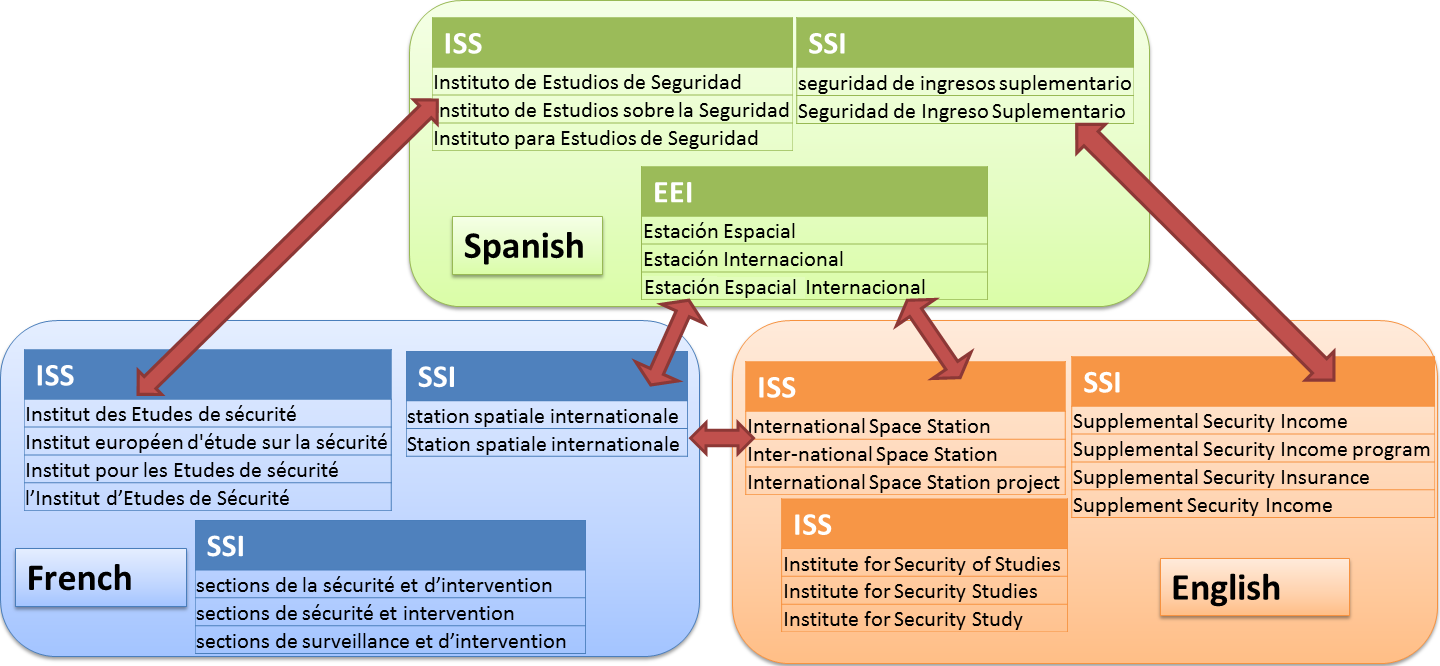
\includegraphics[scale=0.32]{figures/multiLingAcroLinking.png}
\caption{Example of multilingual MWEntity linking}
\label{jac:acronym linking}
\end{figure}


\subsection{Starting point}
\label{jac:starting}

The starting point of our work is a large set of multi-word entities
and their corresponding acronyms in 22 Roman-script languages
\citep{ehrmann-13}. These acronym/expansion pairs were extracted from
the news stream analysed by the EMM processing chain by applying
patterns similar to those proposed by \citet{schwartz-03}. In a
nutshell, the algorithm collects acronym/expansion pairs (such as
\textit{expansion (acronym)} and \textit{acronym (expansion)}) by
identifying short strings within parenthesis, along with candidate
expansions in a side-window of a limited length. A filtering step is
then applied, with the following main constraints: the first letter of
the acronym must be upper-cased, and the length of the expansion must
be smaller than (a) twice as many words as there are characters in the
acronym, or (b) the number of characters in the acronym plus five
words, whichever is the smaller (i.e. $\min(\vert$A$\vert+5,
\vert$A$\vert*2$) words, with $\vert$A$\vert$ being the number of
characters of the acronym). We refer the reader to \citet{schwartz-03}
for more details.  This process resulted in the extraction of 1.7
million expansions for 0.4 million different acronyms.

Applied on news articles, this method identified acronym/expansion
pairs referring mostly to organisation names (e.g.,  \textit{CP} –
\textit{Communist Party}), but also events (\textit{WW2} –
\textit{World War II}), names of drugs or of vaccines (\textit{MMR} –
\textit{measles, mumps, rubella}), organisation types (\textit{NGO} –
\textit{non-governmental organisation}), job titles (\textit{MEP} –
\textit{Member of Parliament}), physical measurement units
(\textit{kmh} – \textit{kilometres per hour}), and more. As one of the
next steps, we will work on categorising the acronym/expansion pairs
into various semantic categories.

To automatically determine which of the expansions are lexical
variants of the same conceptual entity, a clustering step was carried
out, on the basis of expansions having the same language and the same
acronym. This monolingual clustering, based on a pair-wise string
similarity, allowed to distinguish between sets of conceptually
related expansions, such as those referring to the
\textit{International Space Station} and those referring to the
\textit{Institute for Security of Studies}, both clusters having the
acronym \textit{ISS} (cf. \ili{English} part of Figure~\ref{jac:acronym
  linking}).  Evaluated over the 10 most covered languages, this
monolingual clustering has a micro-average precision of 95.2\%
\citep{jacquet-14}.

Out of this monolingual clustering step, we selected only clusters
having at least four expansions, resulting in 81,000 monolingual
clusters with an average of 7.5 expansions per cluster, the biggest
one having 232 expansions.

Based on this data, the objective is to go a step further by
identifying cross-lingual multi-word entity lexical variants. More
specifically, the goal is to link multilingual expansions referring to
the same entity across languages and regardless of their acronyms.  To
this end, we leverage the previously computed monolingual clusters and
attempt to link them across languages. Considering the previous
example with the entity \textit{International Space Station}
(cf. Figure~\ref{jac:acronym linking}), this results in aggregating the
monolingual clusters \textit{SSI-Station spatiale internationale}
(\ili{French}), \textit{ISS-International Space Station} (\ili{English}) and
\textit{EEI-Estaci\'{o}n Espacial} (\ili{Spanish}).  Additionally to linking
expansions across languages and independently from their acronym,
cross-lingual cluster aggregation can also revise monolingual clusters
by aggregating those conceptually related but isolated because of
their acronyms (both pairs \textit{IMF-International Monetary Fund}
and \textit{FMI-Fondo Monetario Internazionale} occur in \ili{Italian}
texts).



\subsection{Approach}
\label{jac:approach}

Cluster aggregation can be cast as the problem of identifying
connected components of a graph, where monolingual clusters represent
vertices and where edges need to be computed.  This section describes
different cross-lingual aggregation strategies tested in our
experiments (cf. Section~\ref{jac:evaluation}) to link sets of monolingual
clusters across languages.

\subsubsection{Cluster aggregation based on common expansions}
\label{jac:aggregation clusters based on common expansions}

The most straightforward solution to link related acronyms in
different langua\-ges (hereafter \textit{ExpAgg}) is to merge those
clusters that have more than \textit{n} expansion forms in common,
independently of whether their acronyms are identical or not (in our
experiments, \textit{n} was set to 1). This aggregation has been
applied both to improve monolingual clusters (cf. IMF vs FMI case
mentioned at the end of Section~\ref{jac:starting}) and to aggregate
clusters across languages.

\subsubsection{Cluster aggregation based on tokens}

\subsubsubsection{Cluster representation}
\label{jac:cluster representation}

For the two following aggregation strategies, monolingual clusters are
no lon\-ger represented by vectors of expansions, but by a vector of all
individual tokens appearing in the expansions.

$C$ is the resulting $(|\mathbb{C}| \times |\mathbb{T}|)$
Cluster-Token matrix where $c_i : i = 1,\ldots{},|\mathbb{C}|$ is a
monolingual cluster, and $t_j : j = 1,\ldots{},|\mathbb{T}|$ is a
token. $\mathbb{T}$ contains all the tokens across languages which
appear at least once in an expansion.  If a token is present in
different languages, such as \textit{place} in \ili{English} and
\textit{place} in \ili{French}, it corresponds to different tokens in
$\mathbb{T}$.

Each token has its own importance to describe a cluster. In order to
compare two clusters on the basis of their most relevant tokens, we
consider the tf-idf value of each token $t_j$ where, in our context,
each cluster $c_i$ is seen as a document and the whole set of clusters
$\mathbb{C}$ as a corpus:
\begin{equation}\label{jac:eq:tfidf}
C(c_i,t_j) = \tf(t_j,c_i) \times \idf(t_j,\mathbb{C})
\end{equation}

\subsubsubsection{Cluster aggregation based on similar tokens}
\label{jac:similar}

This aggregation (hereafter \textit{TokAgg}) addresses cases where 
monolingual clusters do not have identical expansions across languages, but they 
have a significant amount of highly similar tokens.


%\begin{table}
%\centering
%\resizebox{7.0cm}{!} {
%\begin{tabular}{|c|l|c|c|}
%\hline
%Clusters    &  Expansion  & Acronym  &  Language \\\hline \hline
%cluster 1  &  Social-Democratic Party      &  SDP  & en  \\
%                  &  Social Democratic Party      &      &     \\ \hline  
%cluster 2  &  Partito Social-Democratico   &  PSD  & it \\
%                  &  Partito di socialdemocratico &      &    \\
%                  &  Partito socialdemocratico   &       &    \\ \hline
%\end{tabular}}
%\caption{Example of clusters aggregated on the basis of similar tokens}
%\label{jac:tab:common token aggregation}
%\end{table}


\begin{table}[h]
\centering
%\ra{1.1}
%\resizebox{8.5cm}{!}{
\begin{tabular}{clcc}\lsptoprule
Clusters    &  Expansion  & Acronym  &  Language \\
\midrule
cluster 1  &  Social-Democratic Party      &  SDP  & en  \\
                   &  Social Democratic Party      &      &     \\ \midrule
cluster 2  &  Partito Social-Democratico   &  PSD  & it \\
                   &  Partito di socialdemocratico &      &    \\
                   &  Partito socialdemocratico   &       &    \\ 
\lspbottomrule
\end{tabular}
%}
\caption{Example of clusters aggregated on the basis of similar tokens}
\label{jac:tab:common token aggregation}
\end{table}


We compute the matrix $(|\mathbb{T}| \times |\mathbb{T}|)$, hereafter
$\InvEdit$, which corresponds to the inverse of the normalized
Levenshtein edit distance where $t_i : i = 1,\ldots{},|\mathbb{T}|$ and
$t_j : j = 1,\ldots{},|\mathbb{T}|$ are tokens from all the addressed
languages:
\begin{equation}\label{jac:eq:edit}
\InvEdit(t_i,t_j) = 1 - \frac{\Lev(t_i,t_j)}{\max(|t_i|,|t_j|)} 
\end{equation}
$\Lev(t_i,t_j)$ is the Levenshtein edit-distance between $t_i$ and $t_j$, 
and $|t_i|$ and $|t_j|$ are respectively the length of the tokens $t_i$ 
and $t_j$. We filter $\InvEdit$ using a threshold $\delta$ as follows:

\begin{equation}
\InvEdit(t_i,t_j,\delta) =
%\[
\left\{
  \begin{array}{lr}
    \InvEdit(t_i,t_j) & : \InvEdit(t_i,t_j) \ge \delta\\
    0 & : \InvEdit(t_i,t_j) < \delta
  \end{array}
\right.
%\]
\end{equation}

In this case, if $\delta = 1$, $\InvEdit$ only contains values for
exact matching tokens.
This matrix is then used to enrich the monolingual cluster
representation.  Given two languages $l_{1}$ and $l_{2}$, the
corresponding monolingual clusters $C_{l_{1}}$ and $C_{l_{2}}$ do not
have common tokens since in $\mathbb{T}$ tokens are
language-dependent. The $\InvEdit$ matrix is used to identify common or
similar tokens. We convert the obtained matrix $C\_\CTok_{l_{1}}$ to a
binary matrix:

\begin{equation}
C\_\CTok_{l_{1}}(c_i,t_j) =
%\[
\left\{
  \begin{array}{lr}
    1 : C_{l_{1}}(c_i,t_j) \times \InvEdit(c_i,t_j,\delta) > 0\\
    0 : \text{otherwise}
  \end{array}
\right.
%\]
\end{equation}

This aggregation is particularly useful when comparing clusters from
similar languages. Table~\ref{jac:tab:common token aggregation}
illustrates such cases, with the \ili{English}-\ili{Italian} tokens
\textit{Party / Partito} and \textit{Democratic / Democratico}. This
representation can also benefit from the fact that it is possible to
find multi-word entities of a given language in texts in another
language (especially with names of international organisations such as
\textit{European Space Agency} which can be found in \ili{German} text).



\subsubsubsection{Cluster aggregation based on translated tokens}
\label{jac:translated}

%\begin{table}
%\centering
%\resizebox{8.0cm}{!}{
%\begin{tabular}{|c|l|c|c|}
%\hline
%Clusters    &  Expansion  & Acronym  &  Language \\\hline \hline
%cluster 1   &  Russian Academy of Sciences     &  RAS  & en  \\
%                   &  Russian of Academy of Sciences   &         &     \\\hline  
%cluster 2   &  russischen Akademie der Wissenschaften   &  RAW  & de \\
%                   &  Russischen Akademie für Wissenschaften  &          &    \\
%                   &  Russische Akademie der Wissenschaften    &         &    \\\hline
%\end{tabular}}
%\caption{Example of clusters aggregated on the basis of translated tokens}
%\label{jac:tab:translated token aggregation}
%\end{table}

\begin{table}[h]
\centering
%\ra{1.1}
\resizebox{\textwidth}{!}{
\begin{tabular}{clcc}\lsptoprule
Clusters    &  Expansion  & Acronym  &  Language \\
\midrule
cluster 1   &  Russian Academy of Sciences     &  RAS  & en  \\
                    &  Russian of Academy of Sciences   &         &     \\
\midrule
cluster 2   &  russischen Akademie der Wissenschaften   &  RAW  & de \\
                    &  Russischen Akademie für Wissenschaften  &          &    \\
                    &  Russische Akademie der Wissenschaften    &         &    \\
\lspbottomrule
\end{tabular}
}
\caption{Example of clusters aggregated on the basis of translated tokens}
\label{jac:tab:translated token aggregation}
\end{table}


However, many entities have different written forms across languages
so that a string-based comparison of tokens is not successful. We
therefore complement the cluster aggregation by using token
translation probabilities (hereafter \textit{TransTokAgg}).

They are produced using statistical translation models trained on
\isi{parallel corpora} built from Wikipedia, by making use of redirection
tables (i.e.  several written forms redirecting to a specific
page/entity) and of interlingual links between pages (implementation
details of translation models are provided in Section~\ref{jac:trans}).
In order to separate training and test data, any variant name from
these Wikipedia tables matching with one of the 1.7 million expansions
or 0.4 million acronyms is removed from the \isi{parallel corpora} (see
Section~\ref{jac:evaluation}).

Let $\TransMod$ be the resulting $(|\mathbb{T}| \times |\mathbb{T}|)$
\isi{translation model} matrix where $t_i : i = 1,\ldots{},|\mathbb{T}|$ and $t_j
: j = 1,\ldots{},|\mathbb{T}|$ are tokens.  As for $\InvEdit$ matrix, we
filter $\TransMod$ using a threshold $\beta$:

\begin{equation}
\TransMod(t_i,t_j,\beta) =
%\[
\left\{
  \begin{array}{lr}
    \TransMod(t_i,t_j) & : \TransMod(t_i,t_j) \ge \beta\\
    0 & : \TransMod(t_i,t_j) < \beta
  \end{array}
\right.
%\]
\end{equation}

This matrix is then used to enrich the monolingual cluster
representation.  Given a language $l$ and its corresponding
monolingual clusters $C_{l}$,$C\_\TransTok_{l}$ corresponds to the
binary extended matrix based on a given \isi{translation model}:

\begin{equation}
C\_\TransTok_{l}(c_i,t_j) =
%\[
\left\{
  \begin{array}{lr}
    1 : C_{l}(c_i,t_j) \times \TransMod(c_i,t_j,\beta) > 0\\
    0 : \text{otherwise}
  \end{array}
\right.
%\]
\end{equation}

Table~\ref{jac:tab:translated token aggregation} illustrates a case of
such cluster aggregation, thanks to a high score in the $\TransMod$
matrix between tokens \textit{Science} in \ili{English} and
\textit{Wissenschaften} in \ili{German}.

\subsubsection{Aggregation strategies}
\label{jac:aggregation clusters}

 
We formulate cluster linking as the task of identifying connected
components in a graph, where monolingual clusters are vertices and
where edges represent links of related clusters across
languages. Clusters are linked if their similarity is above a certain
threshold $\alpha$. During preliminary experiments, we had also tested
\emph{pure} clustering algorithms, but it turned out that the graph
approach was more efficient.

For the last two cluster aggregation methods (TokAgg and
TransTokAgg), we applied two similarity measures: cosine and
ComMNZ. The latter is actually a data fusion algorithm \citep{fox-94}
which we assimilate, in this context, to a similarity measure.  This
algorithm aims at measuring the similarity between two objects having
multiple comparison criteria. Specifically, the overall similarity
score between two objects is better when those objects have reasonable
similarity scores for all criteria than when they have a very good
similarity score for one criterion, and less good or no value for the
others.  In our case, it would promote the similarity between two
clusters $c_i$ and $c_j$ if they have many similar or translated
tokens $t_k$ with a reasonable similarity score, and it would decrease
the similarity between two clusters $c_i$ and $c_j$ if they have few
similar or translated tokens $t_k$ with a very high similarity score:

\begin{equation}
\CombMNZ(c_i,c_j) = \sum_{t_k\in c_j} \frac{C(c_i,t_k)}{\sum_{t_l\in
    c_i} C(c_i,t_l)} \times \sum_{t_k\in c_j} 1_{\{C(c_i,t_k)\neq0\}}
\end{equation}


\subsection{Evaluation}
\label{jac:evaluation}
\subsubsection{Evaluation dataset}
\label{jac:evalData}

As described in Section~\ref{jac:starting}, the starting point of our
experiments is a set of 81,000 monolingual clusters with one acronym
per cluster, an average of 7.5 expansions per cluster, many of them
having few expansions, and the biggest 232 expansions.

We evaluate cross-lingual cluster aggregation against Wikipedia data
excluding the part used for the translations models (see previous
section).  The gold standard corresponds to a set of Wikipedia
redirection tables and interlingual linking tables, where we consider
Wikipedia entities/pages as cross-lingual classes.  Each class
contains all the expressions listed in the redirection tables in all
the languages linked via the interlingual linking tables. Only classes
having at least two expansions were selected, resulting in a gold
standard of 10,000 classes.  Considering Wikipedia information as a
gold standard is disputable.  The interlingual linkings should be
reliable but this is less the case for the redirection
tables. However, a manual evaluation of the redirection table quality
shows that, in over 160 randomly extracted classes in 4 different
languages (fr, en, de, it), 93.4\% of the forms were correct
\citep{jacquet-14}.

\subsubsection{Parameters}
\label{jac:settings}

Parameters have to be set with regards to, first, the thresholds
$\delta$ and $\beta$ applied to filter out some similarity values in
the above-mentioned token matrices ($C\_\CTok_{l}$ and $C\_\TransTok_{l}$) and, second,
the threshold $\alpha$ applied to the aggregation strategies, i.e. the
one above which clusters are aggregated.

With respect to cluster representations based on similar tokens
$C\_\CTok_{l}$, the threshold $\delta$ should be high in order to
consider two tokens as similar only if they are close in terms of edit
distance. Regarding representations based on translated tokens
$C\_\TransTok_{l}$, the threshold $\beta$ can be low since even a weak
token similarity could be a relevant indicator at the cluster
level. For our experiments, the values of $\delta$ and $\beta$ were
fixed to 0.7 and 0.3 respectively.

Cluster aggregation is allowed when the cluster similarity (either in terms of cosine or
CombMNZ) is above a certain threshold $\alpha$. We experimented with
different values for $\alpha$, ranging from 0.7 to 1 (cf. Section
\ref{jac:results}).

This aggregation step is further regulated with the addition of the
following constraints: two clusters $c_1$ and $c_2$ are linked if
their similarity is above $\alpha$ and if $c_1$ is in the $k$ most
similar clusters of $c_2$ or $c_2$ is in the $k$ most similar clusters
of $c_1$. This additional constraints allow to rule out clusters
having a high similarity with a lot of other clusters.  This is the
case for short and frequent expansions, e.g., \textit{Olympic
  Committee} which is highly similar to a cluster containing
expansions such as \textit{Olympic Organizing Committee} or to another
containing \textit{games organising committee}, but as well to
clusters containing more specific expansions such as \textit{Vancouver
  Olympic Committee}. In our experiments, $k$ equals 3.


\subsubsection{Translation models}
\label{jac:trans}
Cluster representations based on translated tokens correspond to
lexical conditional translation probabilities computed for three
language pairs, between \ili{English} and \ili{French}, \ili{German} and \ili{Italian}. The
translation models were trained on \isi{parallel corpora} built from
Wikipedia, by making use of redirection tables (i.e. several written
forms redirecting to a specific page/entity) and of interlingual links
between pages.  More specifically, given an entity/page $p$ and two
redirection tables $rt_1$ and $rt_2$ in languages $l_1$ and $l_2$,
each written form from $rt_1$ can be seen as a translation $t$ of each
written form from $rt_2$. For a given language pair, the corresponding
parallel corpus is the concatenation of all translations $t$ from all
the entities/pages $p$.

These Wikipedia tables are also used for evaluation purposes (see
Section~\ref{jac:evalData}). As a consequence, the 1.7 million expansions
and 0.4 million acronyms on which the approach is applied were removed
from the \isi{parallel corpora}.

There were about 300,000 training examples for \ili{German}--\ili{English} and
\ili{French}--\ili{English}, and about 170,000 for \ili{Italian}--\ili{English}.  Word
alignments with many-to-one links were generated using the
unsupervised \texttt{fast\_align} tool \citep{dyer-13} in both directions
and combined with the \texttt{grow-diag-final-and} symmetrization
heuristic \citep{koehn-03}. Lexical translation tables for the three
language pairs in both directions where extracted with a tool from the
Moses translation toolkit \citep{koehn2007moses}. Tables contain maximum
likelihood probability estimated for the conditional word translation
probabilities $p(\text{En}|\{\text{Fr},\text{De},\text{It}\})$ and $p(\{\text{Fr},\text{De},\text{It}\}|\text{En})$. Our
$\TransMod$ matrix is constructed based on the concatenation of these
tables.



\subsubsection{Evaluation measures}

Clusters are evaluated against the gold standard using micro-average
Precision and Recall, adopting the mapping between identified clusters
and gold standard clusters which maximised the $F_1$
measure. Micro-average precision (MAV-P) and recall (MAV-R) are
defined as follows:
\begin{equation}
\text{MAV-P} (C) = \frac{\sum_{c \in C}{\EXP(c)_{\text{true}}}}{\sum_{c \in C}{\EXP(c)_{\text{true}}}+\sum_{c \in
 C}{\EXP(c)_{\text{false}}}}
\end{equation}
\begin{equation}
\text{MAV-R} (C) = \frac{\sum_{c \in C}{\EXP(c)_{\text{true}}}}{\sum_{c \in C}{\EXP(c)_{\text{true}}}+\sum_{c \in C}{\EXP(c)_{\text{miss}}}}
\end{equation}
where $C$ is the set of produced clusters, $\EXP(c)_{\text{true}}$ is the set
of expansions in a cluster $c$ which also appear in the corresponding
class of the gold standard, and $\EXP(c)_{\text{false}}$ is the set of
expansions in a cluster $c$ which do not appear in the gold
standard\footnote{We tried two other metrics: macro-average and
  B-cubed measure \citep{bagga-98} but since results are comparable we
  do not report them.}.

\subsubsection{Results and discussion}
\label{jac:results}

%\begin{table}
%\centering
%\resizebox{7cm}{!}{
%\begin{tabular}{|l|c|c|c|}
%\hline
%                                               &  MAV-P  & MAV-R  &  F1 \\ \hline \hline
%Baseline               &     97.7\%   &  51.5\%  & 67.4\%  \\ \hline  
%Monolingual ExpAgg   &  96.8\%   &  54.8\%  & 69.4\%  \\ \hline 
%Multilingual ExpAgg  &     96.9\%   &  65.7\%  & 78.2\%  \\ \hline  \hline  
%Cosine measure                         & & &   \\\hline  \hline  
%TokAgg         &     97.7\%   &  52.5\%  & 68.3\%  \\ \hline  
%TransTokAgg  &     97.6\%   &  51.8\%  & 67.7\%  \\ \hline  
%\textbf{All aggregations}&     \textbf{95.5\%}   &  \textbf{71.4\%}  &  
%\textbf{81.6\%}  \\ \hline  \hline  
%ComMNZ measure                         &    &   &   \\ \hline  \hline  
%TokAgg         &     97.7\%   &  52.5\%  & 68.3\%  \\ \hline  
%TransTokAgg   &     97.7\%   &  51.6\%  & 67.6\%  \\ \hline  
%\textbf{All aggregations}&     \textbf{95.8\%}   &  \textbf{71.2\%}  & 
%\textbf{81.6\%}  \\ \hline  
%\end{tabular}}
%\caption{Cluster aggregation strategies for 3 language pairs}
%\label{jac:tab:Eval3l}
%\end{table}


\begin{table}[h]
\centering
% \ra{1.1}
% \resizebox{7cm}{!}{
\begin{tabular}{lccc}\lsptoprule
&  \textnormal{MAV-P}  & \textnormal{MAV-R}  &  \textnormal{F1} \\ 
\midrule
Baseline                &     97.7\%   &  51.5\%  & 67.4\%  \\  
Monolingual ExpAgg   &  96.8\%   &  54.8\%  & 69.4\%  \\
Multilingual ExpAgg  &     96.9\%   &  65.7\%  & 78.2\%  \\ 
\midrule
\textnormal{Cosine measure}                 & & &   \\
TokAgg          &     97.7\%   &  52.5\%  & 68.3\%  \\   
TransTokAgg  &     97.6\%   &  51.8\%  & 67.7\%  \\  
All aggregations &     \textbf{95.5\%}   &  \textbf{71.4\%}  &  
\textbf{81.6\%}  \\
\midrule
\textnormal{ComMNZ measure}                         &    &   &   \\ 
TokAgg          &     97.7\%   &  52.5\%  & 68.3\%  \\   
TransTokAgg   &     97.7\%   &  51.6\%  & 67.6\%  \\  
All aggregations &     \textbf{95.8\%}   &  \textbf{71.2\%}  & 
\textbf{81.6\%}  \\ 
\lspbottomrule
\end{tabular}
% }
\caption{Cluster aggregation strategies for 3 language pairs}
\label{jac:tab:Eval3l}
\end{table}


Table~\ref{jac:tab:Eval3l} reports the results obtained for the three language pairs 
for which we have a \isi{translation model}, and Table~\ref{jac:tab:Eval22l} reports on a 
global evaluation for 22 languages. In both cases, values were computed with the 
aggregation similarity threshold $\alpha$ set to 0.9.



\begin{table}[h]
\centering
% \ra{1.1}
% \resizebox{7cm}{!}{
\begin{tabular}{lccc}\lsptoprule
&  \textnormal{MAV-P}  & \textnormal{MAV-R}  &  \textnormal{F1} \\ 
\midrule
Baseline                &     98.2\%   &  40.5\%  & 57.4\%  \\ 
Monolingual ExpAgg   &  97.0\%   &  44.9\%  & 60.5\%  \\ 
Multilingual ExpAgg &     97.4\%   &  54.6\%  & 70.0\%  \\ 
\midrule
\textnormal{Cosine measure}                 &    &   &   \\ 
TokAgg          &     98.2\%   &  45.3\%  & 62.0\%  \\  
TransTokAgg  &     97.7\%   &  41.1\%  & 57.9\%  \\
All aggregations &     \textbf{93.1\%}   &  \textbf{65.9\%}  & 
\textbf{77.2\%}  \\
\midrule
\textnormal{ComMNZ measure}                         &    &   &   \\ 
TokAgg          &     98.2\%   &  45.3\%  & 62.0\%  \\ 
TransTokAgg  &     98.2\%   &  40.8\%  & 57.6\%  \\  
All aggregations &     \textbf{95.8\%}   &  \textbf{65.5\%}  & 
\textbf{77.8\%}  \\
\lspbottomrule
\end{tabular}
% }
\caption{Cluster aggregation strategies on 22 languages}
\label{jac:tab:Eval22l}
\end{table}

We defined the baseline as the concatenation of all monolingual
clusters from all languages under consideration. It has a high
precision (97.7\% and 98.2\% in Table~\ref{jac:tab:Eval3l} and
\ref{jac:tab:Eval22l} resp.) and a poor recall (51.5\% and 40.5\%) since
none of the clusters is cross-lingual. The challenge is thus to
improve the recall without affecting the precision too much.

In Tables~\ref{jac:tab:Eval3l} and~\ref{jac:tab:Eval22l}, \textit{monolingual
  ExpAgg} corresponds to the expansion aggregation strategy applied at
the monolingual level, and \textit{multilingual ExpAgg} at the
multilingual level.  The TokAgg and TransTokAgg lines correspond
to results with the corresponding token aggregation strategies using
cosine similarity and CombMNZ fusion, and \textit{All aggregations} to
the ones obtained when using the four aggregation strategies in a
joint way.

It can be observed that each aggregation strategy contributes to
improving the quality of cross-lingual cluster aggregation, with
multilingual ExpAgg providing the best improvement (+10.8 points for
the 3 language pairs and +12.6 points for the 22 languages). The
contribution of the TransTokAgg aggregation is slightly
disappointing; it improves the baseline in both language
configurations, but not significantly.  Nevertheless, when all the
aggregations are applied (bold lines), results are better than the
addition of each single aggregation. It could mean that the
TransTokAgg aggregation provides links between clusters which are
not useful in isolation, but adds relevant bridges between sets of
clusters when combined with other aggregations. Besides, one should
notice that between the three language pairs and the 22 languages,
improvements per aggregation strategy are comparable. Similarly,
results obtained based on cosine similarity and CombMNZ fusion are
comparable.  This strengthens the reliability of the obtained results.

Figure~\ref{jac:fig:Eval22l} shows the impact of the threshold
$\alpha$. When too low (0.7), the F1 measure can be below the baseline
because too many links are established between clusters; when too high
(1.0), aggregations based on similar and translated tokens are reduced
to values close to zero.  In between, it has a clear improvement
impact.

Overall, all aggregations strongly improve the baseline by increasing
the recall (+19.7 and +23.4 points resp.) with a small loss in
precision (\textminus1.9 and \textminus2.4 points resp.). Eventually, there are 64,000
cross-lingual connected clusters across languages instead of 81,000
monolingual ones for the 22 languages.

\begin{figure}
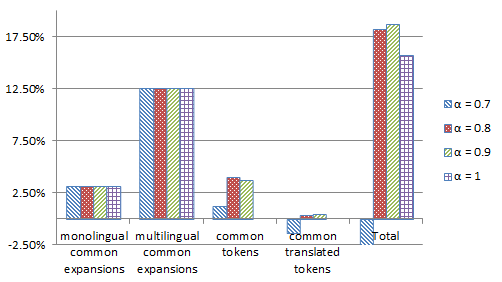
\includegraphics[scale=0.6]{figures/cosine_average_all_ln_improvment1}
\caption{F1 improvement per aggregation type on 22 languages given $\alpha$, using cosine similarity}
\label{jac:fig:Eval22l}
\end{figure}

\section{Multi-word entity pattern learning}
\label{jac:chap10sec4}
The previous section describes an approach which is useful to recognise frequently mentioned MWEntities and cluster them across languages, but it is limited to MWEntities mentioned at least once followed or preceded by its corresponding acronym. In this section we focus on a complementary approach to address the MWEntity recognition task. From the automatically obtained resource composed of 64,000 entities and their 600,000 multilingual lexical variants, we aim at learning MWEntity patterns in order to recognise new and not previously mentioned MWEntities. The described approach is ongoing work. Consequently, if the final goal is to learn these MWEntity patterns from the automatically extracted MWEntity resource, we must first control that our learning approach is reliable independently of the used MWEntity resource's quality. This section describes the use of an existing and reliable resource to evaluate our pattern learning approach.

\subsection{Extraction of organisation names from BabelNet}
\label{jac:sec:babelnet}

For the sake of learning multi-word entity extraction patterns we have exploited BabelNet~\citep{navigli-12},
a large multilingual encyclopedic dictionary and semantic network, created by merging various publicly available linguistic resources, e.g., WordNet and Wikipedia. In particular, BabelNet contains circa 7,7 millions of named entity-related (NE-related) synsets. We used the BabelNet API\footnote{\url{http://babelnet.org/guide}} to extract organisation names for \ili{English} and \ili{Spanish}, which were then used in the process of learning patterns in various ways. Since the NE-related BabelNet synsets are not tagged with a specific NE tag, the NE type was inferred through utilisation of the hypernym information provided in BabelNet (i.e., using WordNet hypernyms and Wikipedia categories). To be more precise, based on hypernym frequency information for the entire set of named entities a list of \textit{positive} (circa 200) and \textit{negative} (circa 20) hypernyms was manually created. These lists were subsequently used to extract organisation names, i.e., a given synset was extracted if: (a) there was at least one hypernym for the main sense of the synset in the list of positive hypernyms, and (b) no hypernym for the main sense of the synset was on the list of negative hypernyms. For instance, the list of positive hypernyms for extracting organisations includes terms like: \textit{airline}, \textit{enterprise}, \textit{corporation}, \textit{bank}, \textit{local\_government}, \textit{political\_organisation}, \textit{law\_enforcement\_agency}, whereas the list of negative hypernyms includes terms like \textit{person} and \textit{human}. The main drive behind the usage of negative hypernym list was to filter out potentially ambiguous named entity candidates. In total, we have extracted 647 898 and 127 264 organisation names for \ili{English} and \ili{Spanish} respectively. We exploited only names that consisted of at least two tokens for the multi-word organisation name pattern learning, which resulted in maintaining only 87.0\% (557 841) of the \ili{English} and 86.1\% (127 264) of the \ili{Spanish} organisation names extracted. Noteworthy, the resource for \ili{English} obtained in this manner includes a portion of organisation names in foreign languages, which is most likely due to the fact that some non-\ili{English} name variants have been tagged in BabelNet as variants in \ili{English}. Since the entire procedure for pulling out organisation names from BabelNet is automated such language-specific name variants have not been manually removed.

\subsection{Learning multi-word entity patterns based solely on BabelNet resources}
\label{jac:sec:babelnet-only-derived-patterns}

The first approach to learning multi-word organisation name extraction patterns exploits as the only resource the organisation names extracted from BabelNet (see Section~\ref{jac:sec:babelnet}). Therefrom, simple linear patterns are learned that consist of two types of elements, namely, surface forms (as they appear in the organisation names) and generic token classes, which will be referred to as token class elements. Example (\ref{jac:exUniversity}) illustrates the syntax of the patterns.

%\begin{verbatim}
\ea\label{jac:exUniversity}
    \texttt{University [] of [] the [] [UPP\_W] [] in [] [UPP\_W]} \\
    \texttt{[ALLCAP] [] [UPP\_W] [] Construction [] Group} \\
    \texttt{The [] [NUM\_LET] [] Company} \\
    \texttt{[UPP\_W] [DASH] Institute}
\z
%\end{verbatim}

\noindent \verb+[]+ denotes a whitespace (not necessarily required to be included in the pattern as illustrated by the last pattern), whereas other token classes are delimited using square brackets. There are 28 generic token classes, out of which 8 cover natural language words (e.g., \verb+[UPP_W]+ - uppercase word, \verb+[LOW_W]+ - lowercase word, \verb+[ALLCAP]+ - all capital words), letters (e.g., \verb+[SINGCAP]+ - single capital letter), numbers (e.g., \verb+[NUM]+) and combinations thereof (e.g., \verb+[NUM_LET]+ - sequence of digits followed by a sequence of letters, etc.), whereas the remaining 20 classes are used to denote specific symbols (e.g., brackets, commas, dots, colons, etc.). 

The pattern learning process consists of three main steps: (a) acquisition of candidate patterns, (b) filtering unreliable and ambiguous candidate patterns, and (c) ranking patterns. These are described in more detail below.

%\vspace{0.3cm}
%\noindent
\subsubsection{Acquisition of candidate patterns} First, each organisation name is transformed into a candidate pattern, i.e., each token which can be found in a set of predefined surface forms (consisting of keywords that trigger organisation names, e.g.,  \textit{University}, and frequently occurring word forms, e.g., prepositions) remains unchanged, whereas all other tokens are mapped into a corresponding generic token class. Each candidate pattern must contain at least one surface form and at least one token-class element,
otherwise it is discarded.

The set of predefined surface forms has been computed automatically and consists of word uni-grams that fulfill the following criteria: (a) it appears more than $\phi=20$ times as part of an organisation name, (b) it does not appear on a list of known toponyms\footnote{We used GeoNames resource at: \url{http://www.geonames.org} for this purpose.}, (c) it does not appear on the list of known first names and surnames\footnote{We used for this purpose {\sc JRC Name Variant Database} and huge list of first names extracted from~\cite{piskorski-11}}, and (d) it is not an adjective (unless it appears very frequently). For instance, for the subset of \ili{English} organisation names consisting solely of company names, the 10 top-most frequent word uni-grams that fulfill the aforementioned criteria are: \textit{Company}, \textit{and}, \textit{of}, \textit{The}, \textit{Group}, \textit{Corporation}, \textit{Bank}, \textit{de}, \textit{Limited} and \textit{Air}.  

%\vspace{0.3cm}
%\noindent
\subsubsection{Filtering candidate patterns} In the subsequent
step, a candidate pattern is discarded if:
\begin{enumerate}
\item its final element is the token class \verb+[LOW_W]+ (any
  lowercase word), or
\item it contains only surface forms which are single uppercase
  letters and it does not contain any token-class element representing
  words starting with an uppercase letter (e.g., \verb+[UPP_W]+,
  \verb+[ALLCAP]+), or
\item it starts with an initial uppercase letter, followed by an
  optional dot and a sequence of token classes corresponding to words
  starting with uppercase letters (and \isi{variations} of this pattern),
  e.g., the following candidate pattern would be discarded:
  \verb+A [] [DOT] [] [UPP_W] [] [ALLCAP]+
\end{enumerate} 

%\noindent
The filtering rules 1--2 are used in order to eliminate
unreliable patterns, i.e., ones that are likely to overgenerate,
whereas the filtering rule 3 aims at eliminating candidate patterns
that are likely to match person names.  The application of the
filtering resulted in maintaining 47,496 (12,966) extraction patterns
for \ili{English} (\ili{Spanish}), where 32.3\% (41.9\%) of these patterns were
observed more than once. Interestingly, only 0.57\% of \ili{English} and
0.35\% of the \ili{Spanish} patterns occur more than 
100 times.

%\vspace{0.3cm}
%\noindent
\subsubsection{Ranking patterns} In the final step candidate patterns are ranked with respect to their reliability based on the
following general assumptions related to their structure: 
\begin{itemize}
\item a pattern that contains either: (a) a larger fraction of surface forms vis-a-vis token-class elements, or (b) longer sequences of consecutive surface forms is deemed more reliable,
\item a pattern whose final element is a lowercase surface form is deemed less reliable,
\item a pattern that contains either: (a) a larger fraction of token-class elements representing single capital letters and lowercase words,
or (b) longer sequences of consecutive token-class elements representing lowercase words is deemed less reliable.
\end{itemize}

%\noindent
The formal definition of the reliability score ($\Rel(p)$) for a pattern $p$ is given below, where the expressions starting with $\#$ denote the number of elements in the pattern of a specific type\footnote{$\#\text{LowerCTokens}(p)$ denotes the number of lowercase tokens, while $\#\text{NonWhitespaces}(p)$ denotes the number of elements in the pattern which are not whitespaces, i.e., it is a count of surface forms and token-class elements. $\text{LastElementIsLowercaseToken}(p)$ denotes a function which returns 1 in case the last element of the pattern is a lowercase token class or 0 otherwise.} and $\alpha=0.2$, $\beta=0.2$, $\gamma=0.2$, $\delta=0.15$, $\lambda=0.1$ and $\kappa=0.15$ are weighting coefficients for the various criteria used in the reliability ranking, whose values have been set based on empirical observations.  
\begin{eqnarray*}
\Rel(p) & = & \frac{\#\text{SurfaceForms}(p) \cdot \alpha +
  \#\text{ConsecutiveSurfaceForms}(p) \cdot \beta}{\#\text{NonWhitespaces}(p)} \\ &
- & \frac{(\#\text{LowerCTokens}(p) \cdot \gamma +
  \#\text{ConsecutiveLowerCTokens}(p) \cdot \delta)}{\#\text{NonWhitespaces}(p)}\\ &
- & \frac{\#\text{SingleCapitalLetterTokens}(p) \cdot
  \lambda}{\#\text{NonWhitespaces}(p)}\\ & + & \gamma + \delta + \lambda + (1
- \text{LastElementIsLowerCToken}(p)) \cdot \kappa \\
\end{eqnarray*}
%\noindent
A few examples of patterns with various reliability scores
(provided in brackets) are given below.

{\small
\begin{verbatim}
    Ministry [] of [] Foreign [] Affairs [] of [] [UPP_W]          (0.97)
    Institute [] of [] [UPP_W] [] Studies                          (0.95)
    [UPP_W] [] [UPP_W] [] [ALLCAP] [] at [] [UPP_W] [] University  (0.67)
    St [DOT] [] [LOW_W] [] [LOW_W] [] [LOW_W] [] [LOW_W] [] school (0.24)
    [UPP_W] [] [LOW_W] [] [LOW_W] [] [LOW_W] [] committee          (0.22)
\end{verbatim}
}

Figure~\ref{jac:pattern-distr} depicts the distribution of patterns with
respect to their reliability scores.

\begin{figure}
\centering
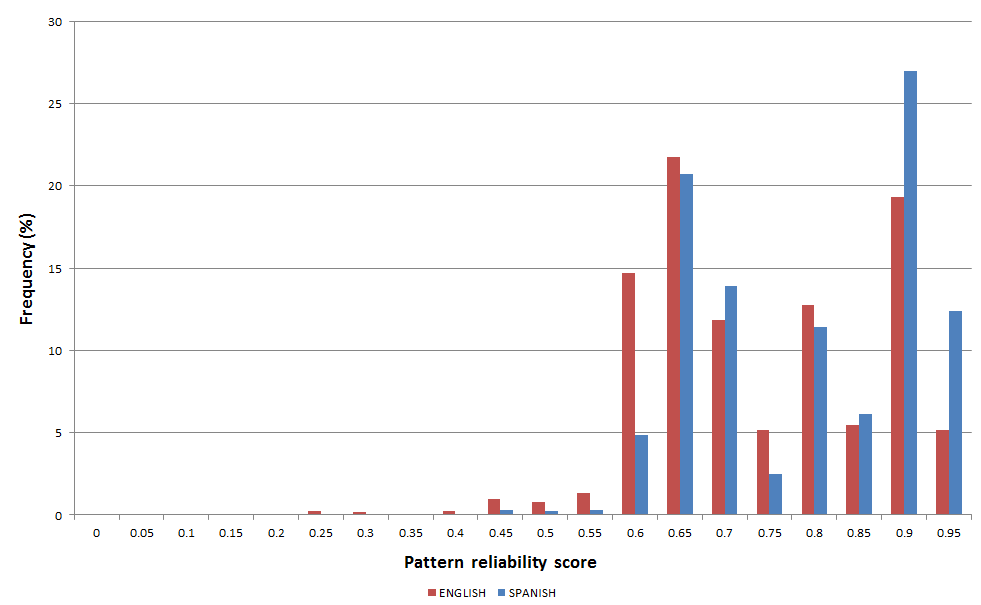
\includegraphics[width=.95\textwidth]{figures/patterns-distr.png}
\caption{\label{jac:pattern-distr}Distribution of patterns with respect to their reliability score for English and Spanish. Each of the bars represents the fraction of patterns, whose reliability score is within the range $(x,x+0.5>$, where $x \in \{0,0.5,\ldots{},0.95\}$.\todo[inline]{Please check the expression $(x,x+0.5>$, esp. the closing angle bracket}}
\end{figure}

\subsection{Evaluation}
In order to evaluate the quality of the learned patterns we used two NE annotated corpora from the CoNLL shared task for \ili{English} and \ili{Spanish}\footnote{\url{http://www.cnts.ua.ac.be/conll2002/ner/} and \url{http://www.cnts.ua.ac.be/conll2003/ner/}}, which contains respectively 6,300 and 7,389 organisation occurrences, and tested the performance using different settings. In particular, we compared three settings: (a) using only BabelNet-derived patterns (denoted in the figures with \textsc{patterns}),  (b) using only an existing rule-based \textsc{ner} system as a baseline (denoted \textsc{rules}), (c) combining rule-based \textsc{ner} system and BabelNet-derived patterns (denoted in the figures with \textsc{rules+patterns}).
In our experiments, we used an in-house rule based \textsc{ner} system \citep{steinberger-11, ehrmann-15} that is geared towards high precision. The choice of a specific \textsc{ner} system is not decisive for these experiments, but by combining an existing \textsc{ner} system with our BabelNet-derived patterns, we aim at testing how our automatically created patterns could be useful to improve the quality of the \textsc{ner} recognition.

Figures~\ref{jac:fig:eval_patterns_english_precision},~\ref{jac:fig:eval_patterns_english_recall},~\ref{jac:fig:eval_patterns_spanish_precision}
and~\ref{jac:fig:eval_patterns_spanish_recall} depict the performance of applying the BabelNet-derived patterns for \ili{English} and \ili{Spanish} 
in terms of precision and recall. The precision and recall values were computed for the varying minimum pattern reliability threshold in the range of $\{0.10,0.15,\ldots{},0.95\}$, i.e., patterns below the minimum reliability threshold were discarded.
The figures are showing the results obtained for exact matching (denoted with \textsc{exact}-\textsc{patterns} or \textsc{exact}-\textsc{rules+patterns}) and for fuzzy matching, e.g., when there is a matching but with a left or right boundary mismatch (denoted with \textsc{fuzzy}-\textsc{patterns} or \textsc{fuzzy}-\textsc{rules+patterns}).
We did not visualise the results corresponding to the \textsc{rule} setting in the figures because they do not depend on the reliability threshold. However, the obtained scores for this setting are embraced in Table~\ref{jac:tab:EvalPatterns}.

\begin{figure}
\centering
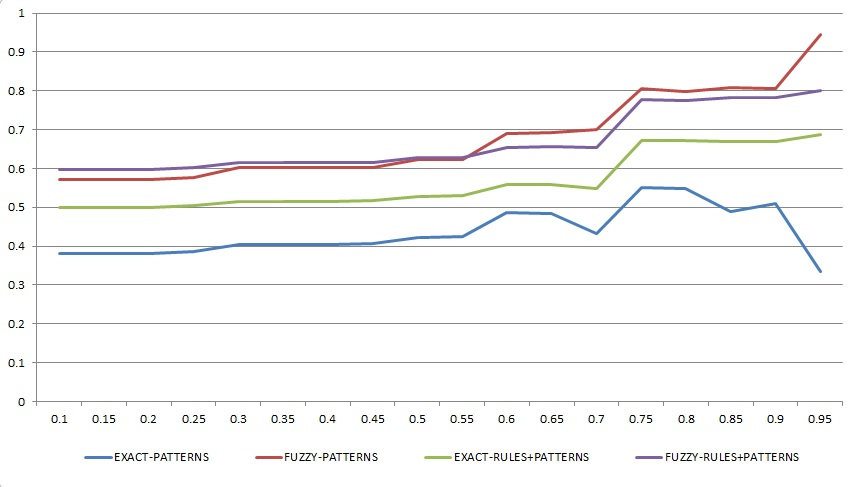
\includegraphics[width=.95\textwidth]{figures/eval_patterns_English_precision.jpg}
\caption{Experiments on English: Precision curves reflecting the performance of applying BabelNet-derived patterns and combining them with a rule-based \textsc{ner} system}
\label{jac:fig:eval_patterns_english_precision}
\end{figure}

\begin{figure}
\centering
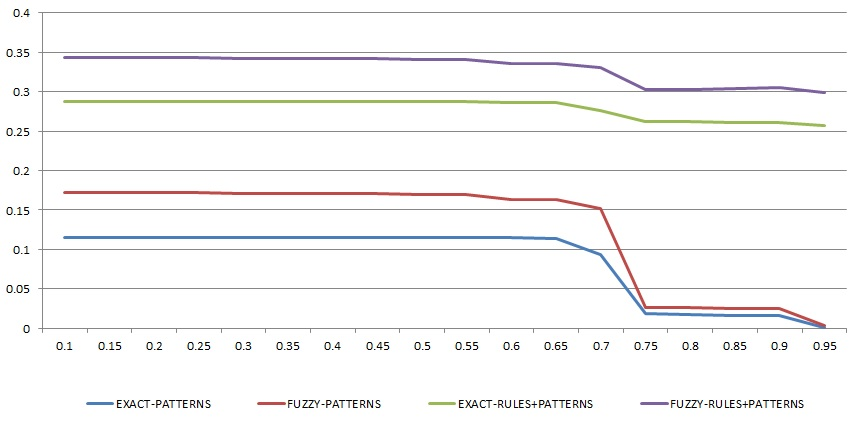
\includegraphics[width=.95\textwidth]{figures/eval_patterns_English_recall.jpg}
\caption{Experiments on English: Recall curves reflecting the performance of applying BabelNet-derived patterns and combining them with a rule-based \textsc{ner} system}
\label{jac:fig:eval_patterns_english_recall}
\end{figure}

\begin{figure}
\centering
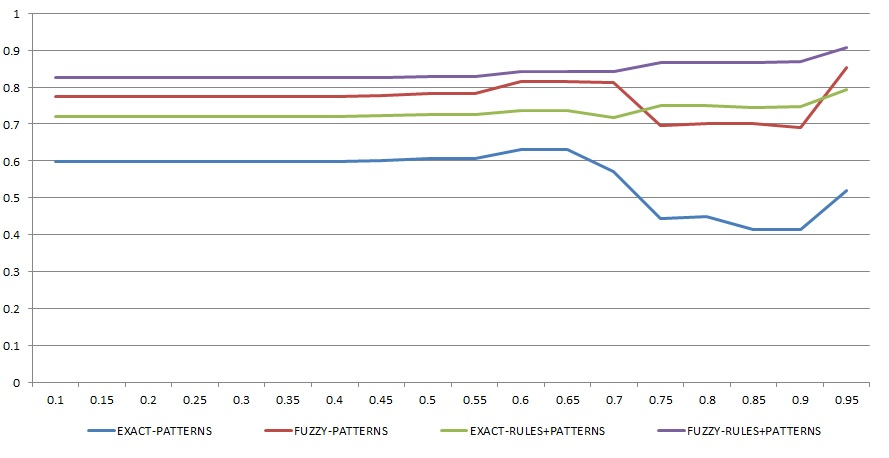
\includegraphics[width=.95\textwidth]{figures/eval_patterns_Spanish_precision.jpg}
\caption{Experiments on Spanish: Precision curves reflecting the performance of applying BabelNet-derived patterns and combining them with a rule-based \textsc{ner} system}
\label{jac:fig:eval_patterns_spanish_precision}
\end{figure}

\begin{figure}
\centering
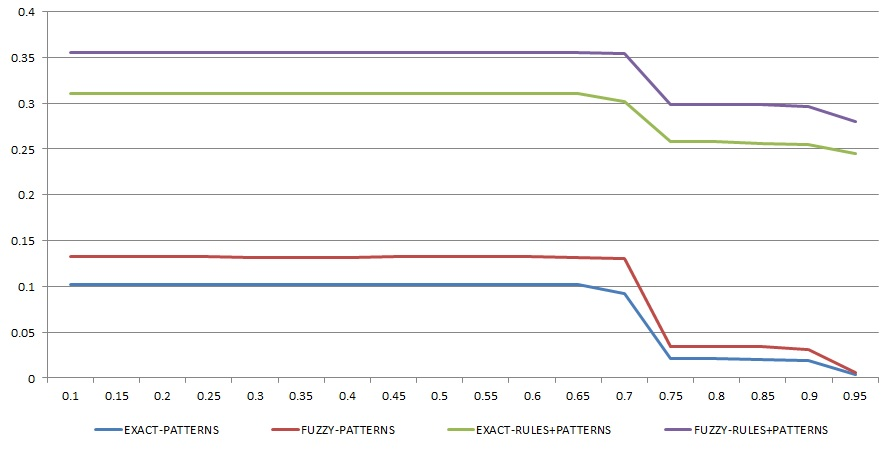
\includegraphics[width=.95\textwidth]{figures/eval_patterns_Spanish_recall.jpg}
\caption{Experiments on Spanish: Recall curves reflecting the performance of applying BabelNet-derived patterns and combining them with a rule-based \textsc{ner} system}
\label{jac:fig:eval_patterns_spanish_recall}
\end{figure}
        
Table~\ref{jac:tab:EvalPatterns} provides the results obtained with a pattern-reliability threshold equal to 0.60, which corresponds to the best results obtained in both languages. For the \textsc{exact} evaluation, an improvement in terms of F1 of 6.5 points for \ili{Spanish} could be observed with the setting \textsc{rules+patterns} versus the baseline \textsc{rules}. As regards \textsc{fuzzy} evaluation, one could observe an improvement of F1 of 7.6 and 1.1 points for \ili{Spanish} and \ili{English} respectively when comparing \textsc{rules+patterns} versus the baseline \textsc{rules} setting.


\begin{table}[h]
\begin{tabular}{l ccc ccc}\lsptoprule
&     \multicolumn{3}{c}{\textsc{exact} matching}  & \multicolumn{3}{c}{\textsc{fuzzy} matching}  \\\cmidrule(lr){2-4}\cmidrule(lr){5-7}
&  \textbf{P}  & \textbf{R}  &  \textbf{F1}  &  \textbf{P}  & \textbf{R}  &  \textbf{F1} \\ 
\midrule
\textnormal{Spanish}                        & & &  & & &   \\
\textsc{patterns}                &     63.1\% & 10.2\% & 17.6\% & 81.4\% & 13.2\% & 22.8\%  \\  
\textsc{rules}   &  \textbf{79.8\%} & 24.2\% & 37.1\% & \textbf{91.3\%} & 27.6\% & 42.4\%  \\
\textsc{rules+patterns}  &     73.5\% & \textbf{31.0\%} & \textbf{43.6\%} & 84.2\% & \textbf{35.5\%} & \textbf{50.0\%}  \\ 
\midrule
\textnormal{English}                        & & & &  & &   \\
\textsc{patterns}                &     48.5\% & 11.4\% & 18.5\% & 69.2\% & 16.3\% & 26.4\%   \\  
\textsc{rules}   &  \textbf{69.0\%} & 25.5\% & 37.3\% & \textbf{80.4\%} & 29.7\% & 43.4\%  \\
\textsc{rules+patterns}  &     55.9\% & \textbf{28.7\%} & \textbf{37.9\%} & 65.6\% & \textbf{33.6\%} & \textbf{44.5\%}  \\ 
\lspbottomrule
\end{tabular}
\caption{Results obtained with pattern reliability threshold = 0.60}
\label{jac:tab:EvalPatterns}
\end{table}


\subsubsection{Mistakes and fuzzy matchings}
\todo[inline]{This subsubsection is the only subsection to ``Evaluation''}
Using existing NE annotated corpora for our preliminary experiments was the most obvious choice to measure the quality of our patterns. Nevertheless, it appears that some MWEntities recognised by the BabelNet-derived patterns considered as incorrectly extracted according to the annotated corpora, could still be considered as correct extractions.
Figure~\ref{jac:fig:error_analysis} provides the complete list of 'wrong' MWEntities (first column) recognised by our patterns when pattern reliability threshold equals 0.90. Even if some cases are clear mistakes, like \textit{Results of European Super} or \textit{Bank on Thursday}, large fraction of the extractions could be considered as valid organisation names. The two other columns show the partial matches with the same reliability threshold, which are considered as incorrect in the \emph{Exact matching} evaluation, and correct in the \emph{Fuzzy matching} evaluation. Again, if some of them are clear mismatches, like \textit{European Commission on Wednesday} or \textit{NATO and the European Union}, most of the extractions appear to be consistent entities.

We expect to achieve higher precision of the learned patterns through
embracing in the computation of the reliability score additional
external evidence, i.e., exploiting contextual information obtained
from pattern matchings in a web-scale corpus to judge the correctness.

\begin{figure}
\centering
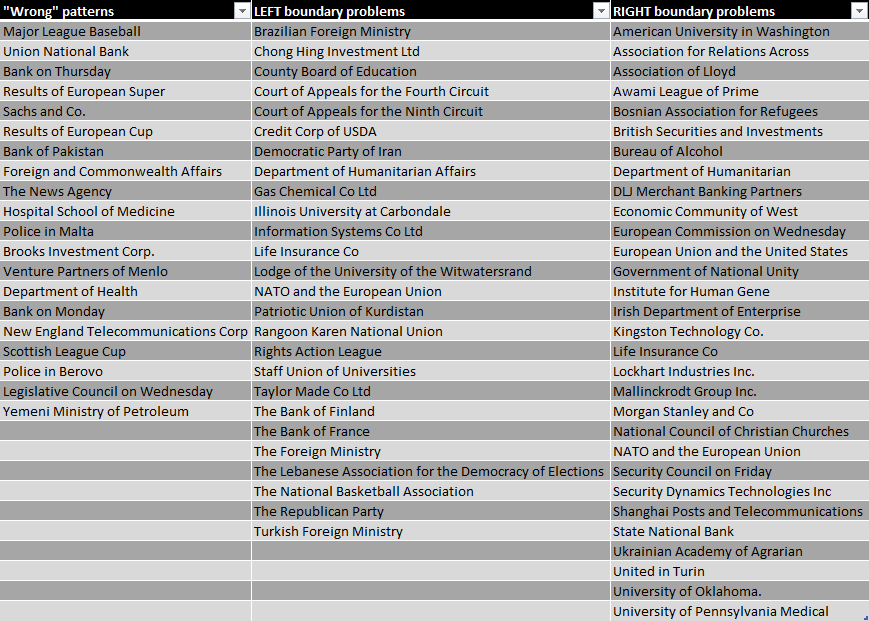
\includegraphics[scale=0.54]{figures/error_analysis.png}

\caption{Complete list of 'wrong' MWEntities and left or right boundary mismatching with pattern reliability threshold = 0.90}
\label{jac:fig:error_analysis}
\end{figure}


\section{Conclusion and future work}
The methods described in this chapter have produced a large 22-language resource containing Multi-word entities of different types and a number of automatically learned patterns to recognise newly occurring MWEntities. We intend to integrate these recognition patterns, together with the variant matching techniques, into the workflow of the Europe Media Monitor. An interesting feature of this collection and the patterns is that all MWEntity forms were found in real-world text and that large numbers of variants were identified, including typos, simplifications of longer names, syntactic and morphological variants and translational equivalences.

The results obtained in MWEntity recognition with the patterns automatically derived from BabelNet are promising when applied to \ili{English} and \ili{Spanish}, although the reported approach and evaluation figures reflect only our preliminary research in this area. Expanding the pattern learning to other languages is part of our future work. We also envisage applying the same pattern learning approach from the automatically created MWEntity resource. This would require to categorise the MWEntity sets into some broad semantic classes (e.g., organisations, events, measurements, and others) which is a task we are currently working on.

Furthermore, we are also working on expanding the patterns we learned based on a distributional approach. It consists of replacing meaningful surface forms from each pattern by a cluster of surface forms that would belong to the same semantic class. In such a way, similar words like \textit{company}, \textit{firm}, \textit{corporation}, etc., will be part of the same cluster because they have a high distributional similarity. Finally, the pattern reliability scoring could be extended through inclusion of additional statistics when applying the patterns on web-scale corpora.

%\section*{Abbreviations}
%\section*{Acknowledgements}

{\sloppy\printbibliography[heading=subbibliography,notkeyword=this]}

\end{document}
